\newpage
\subsection{Digital Twin}
Ein digitaler Nachbau der in der Aufgabenstellung beschriebenen Gegebenheiten bietet vielfältige Vorteile. Dazu zählt die Möglichkeit, potenzielle Probleme frühzeitig zu identifizieren, noch bevor physische Produkte beschafft werden müssen. Zudem kann eine solche Visualisierung zur Generierung von Trainingsdaten für Bildverarbeitungssysteme beitragen. Die Unreal Engine, ursprünglich als 3D-Spiele-Engine entwickelt, hat sich mittlerweile in zahlreichen Anwendungsbereichen etabliert und ermöglicht die effiziente Erstellung virtueller Umgebungen sowie die dynamische Bewegung von Objekten in diesen Welten. Durch die Verwendung von Bildern des Mensabodens, die präzise Modellierung von Hindernissen und Pylonen sowie den Einsatz einfacher Skripte, kann eine realitätsnahe Testumgebung mit hoher Genauigkeit nachgebildet werden.

\begin{figure}[h!]
    \centering
    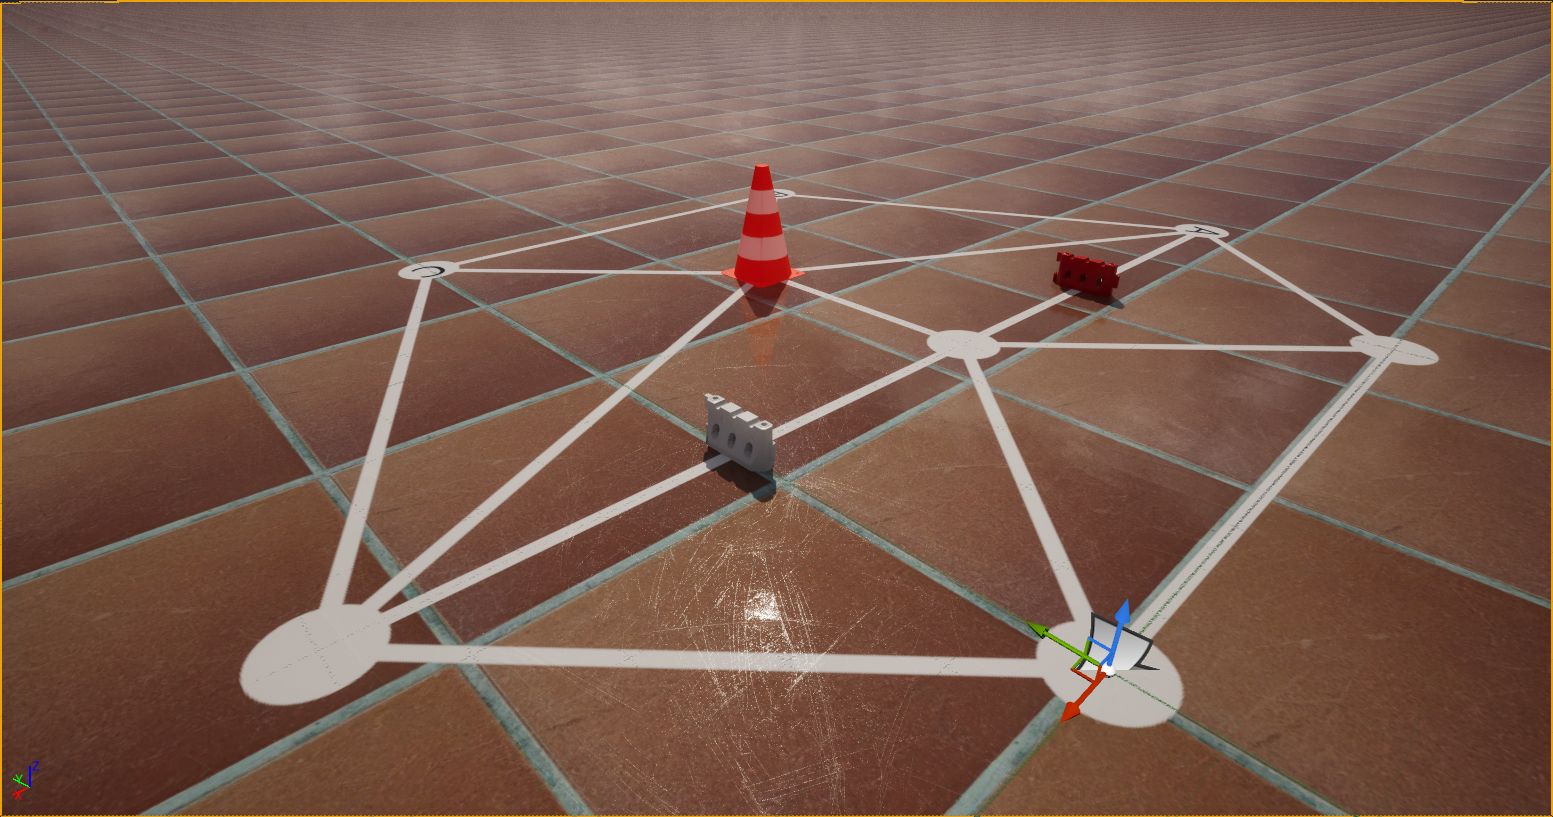
\includegraphics[width=0.9\textwidth]{img/unrealengine/overview.png}
    \caption{Übersicht Unreal Engine}
\label{img:Übersicht Unreal Engine}
\end{figure}
\subsubsection{Kamera-Konfiguration}
Der Digital Twin erlaubt das einfache Testen von verschiedenen Kamera-Konfigurationen. Unter anderem Das Kamera-Sichtfeld, sowie verschiedene Neigungswinkel. In folgender Tabelle sind die Ergebnisse unterschiedlicher Kamerakonfigurationen zu sehen.
\begin{table}[H]
    \centering
    \begin{tabular}{|c|c|c|c|}
        \hline
        & Höhe 30cm & Höhe 50cm & Höhe 75cm \\
        \hline
        \parbox[c][2cm][c]{4cm}{\centering Kamera FoV 75°, \\ Kameraneigung 30°} & 
        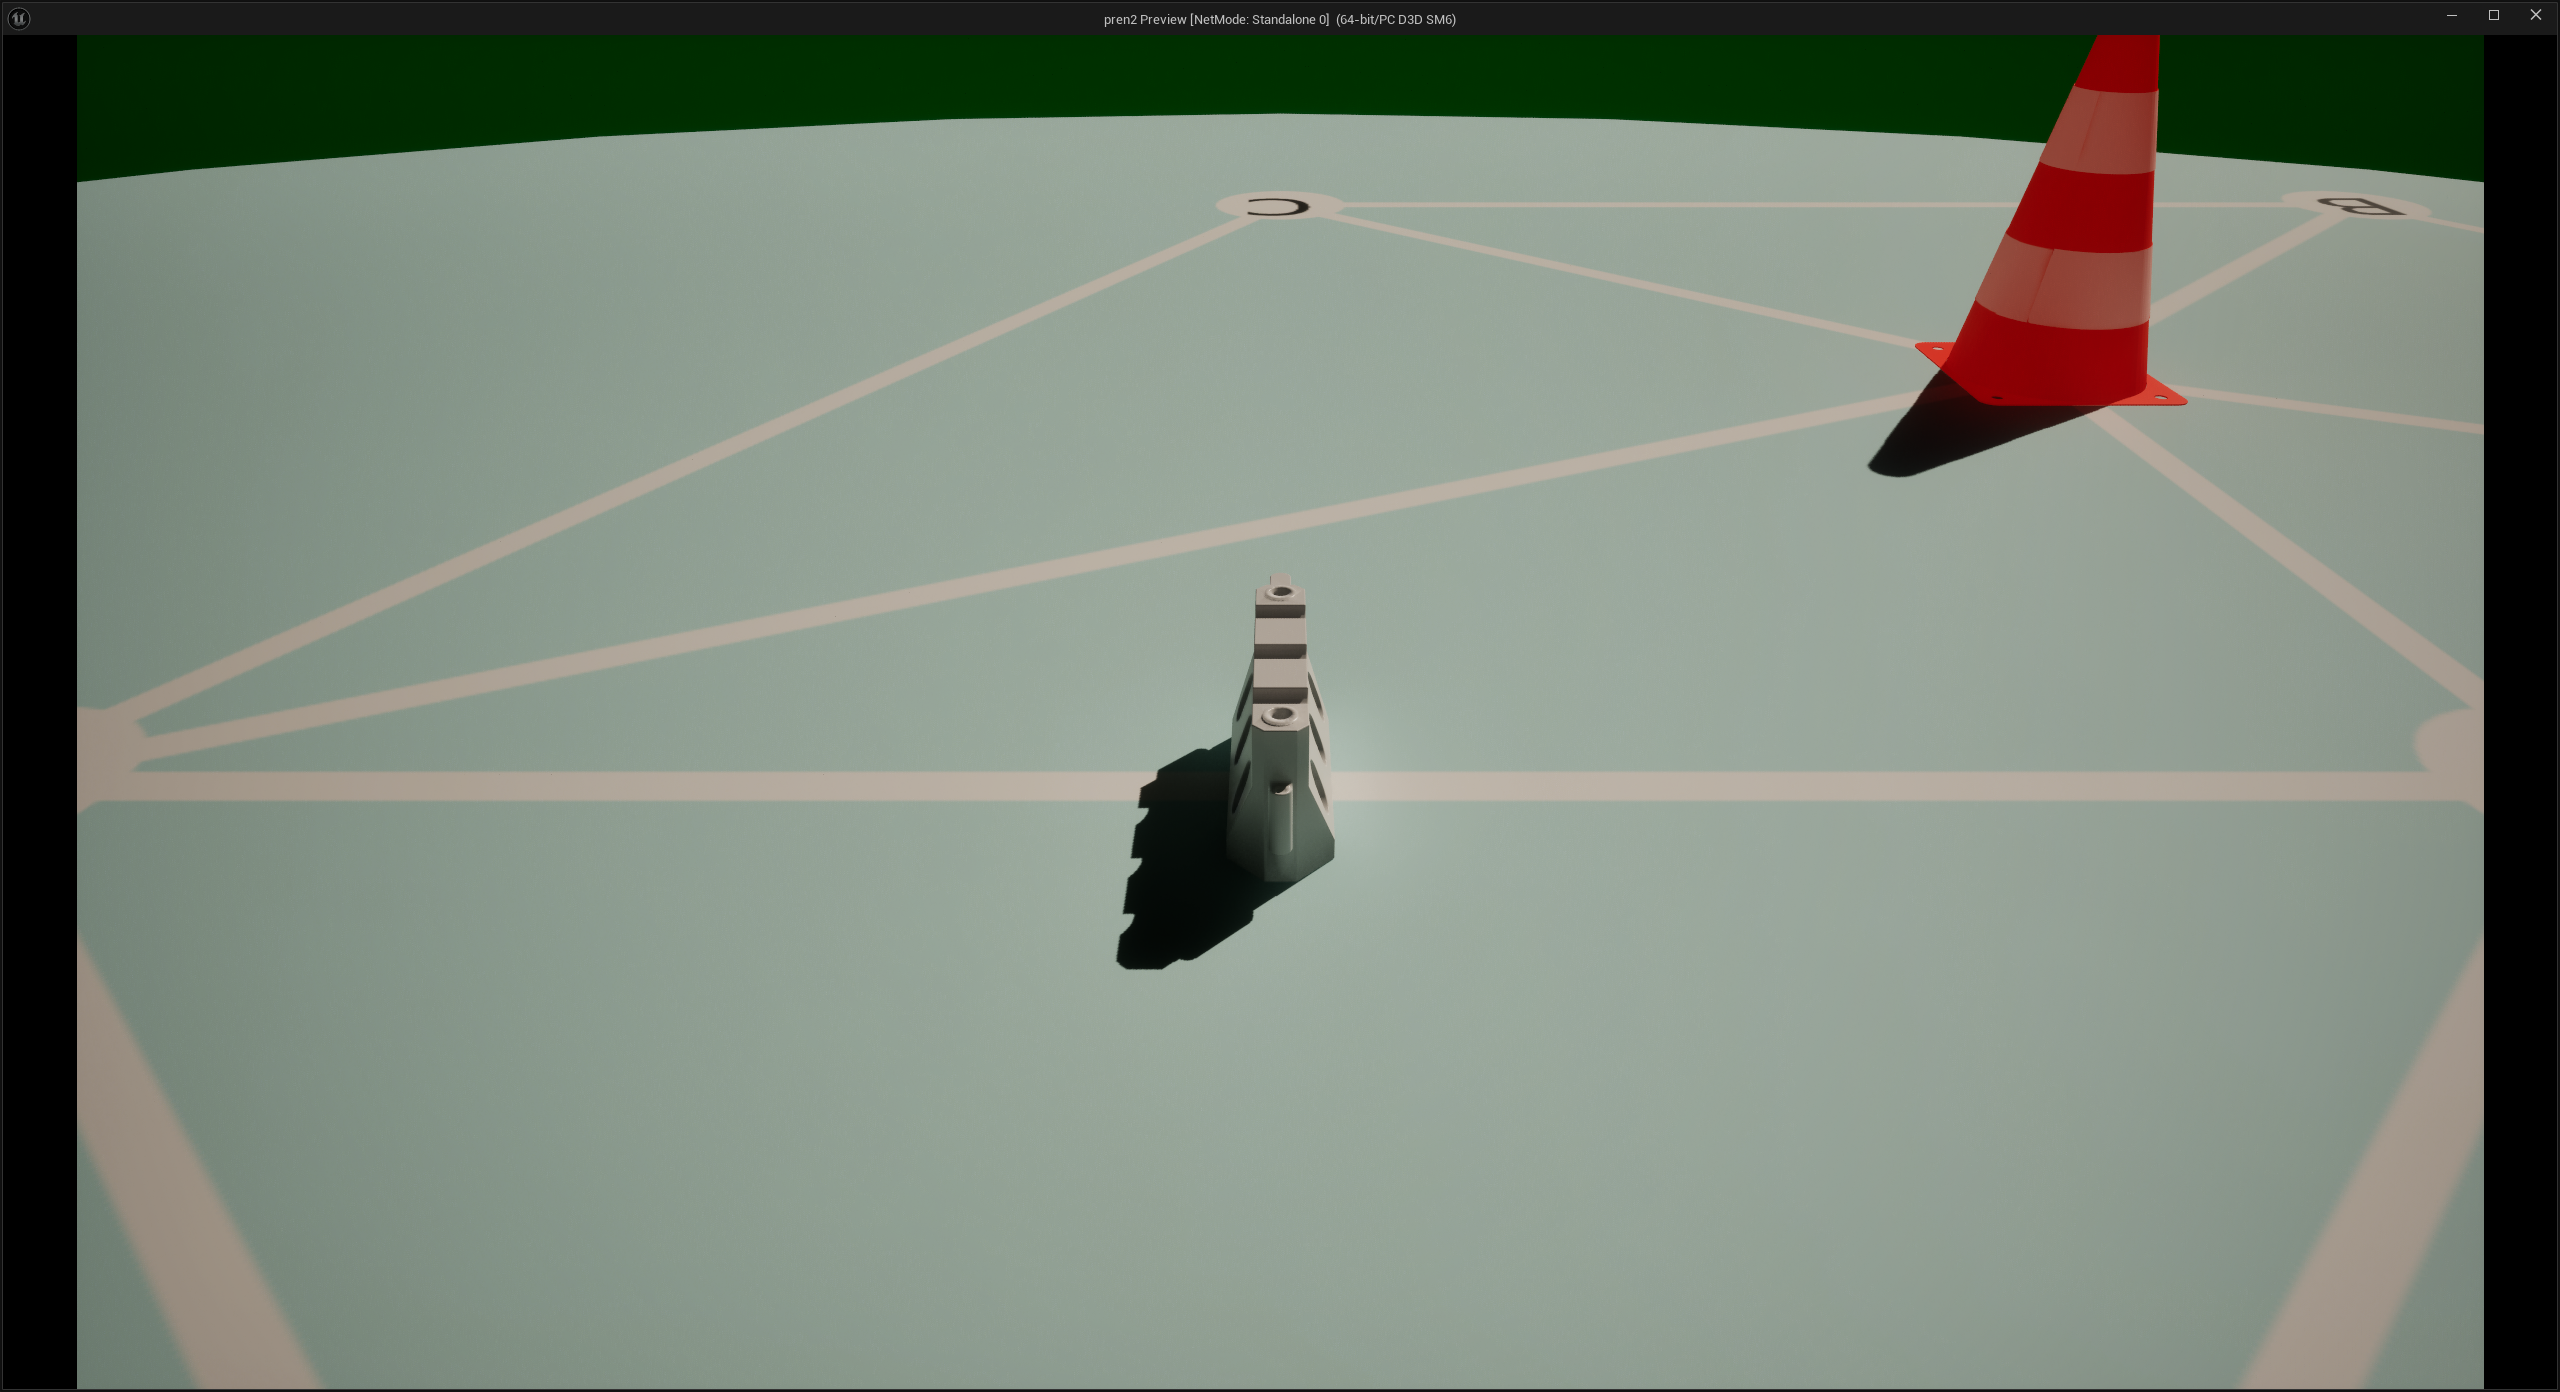
\includegraphics[width=4cm]{img/unrealengine/h30_f75_w30.png} & 
        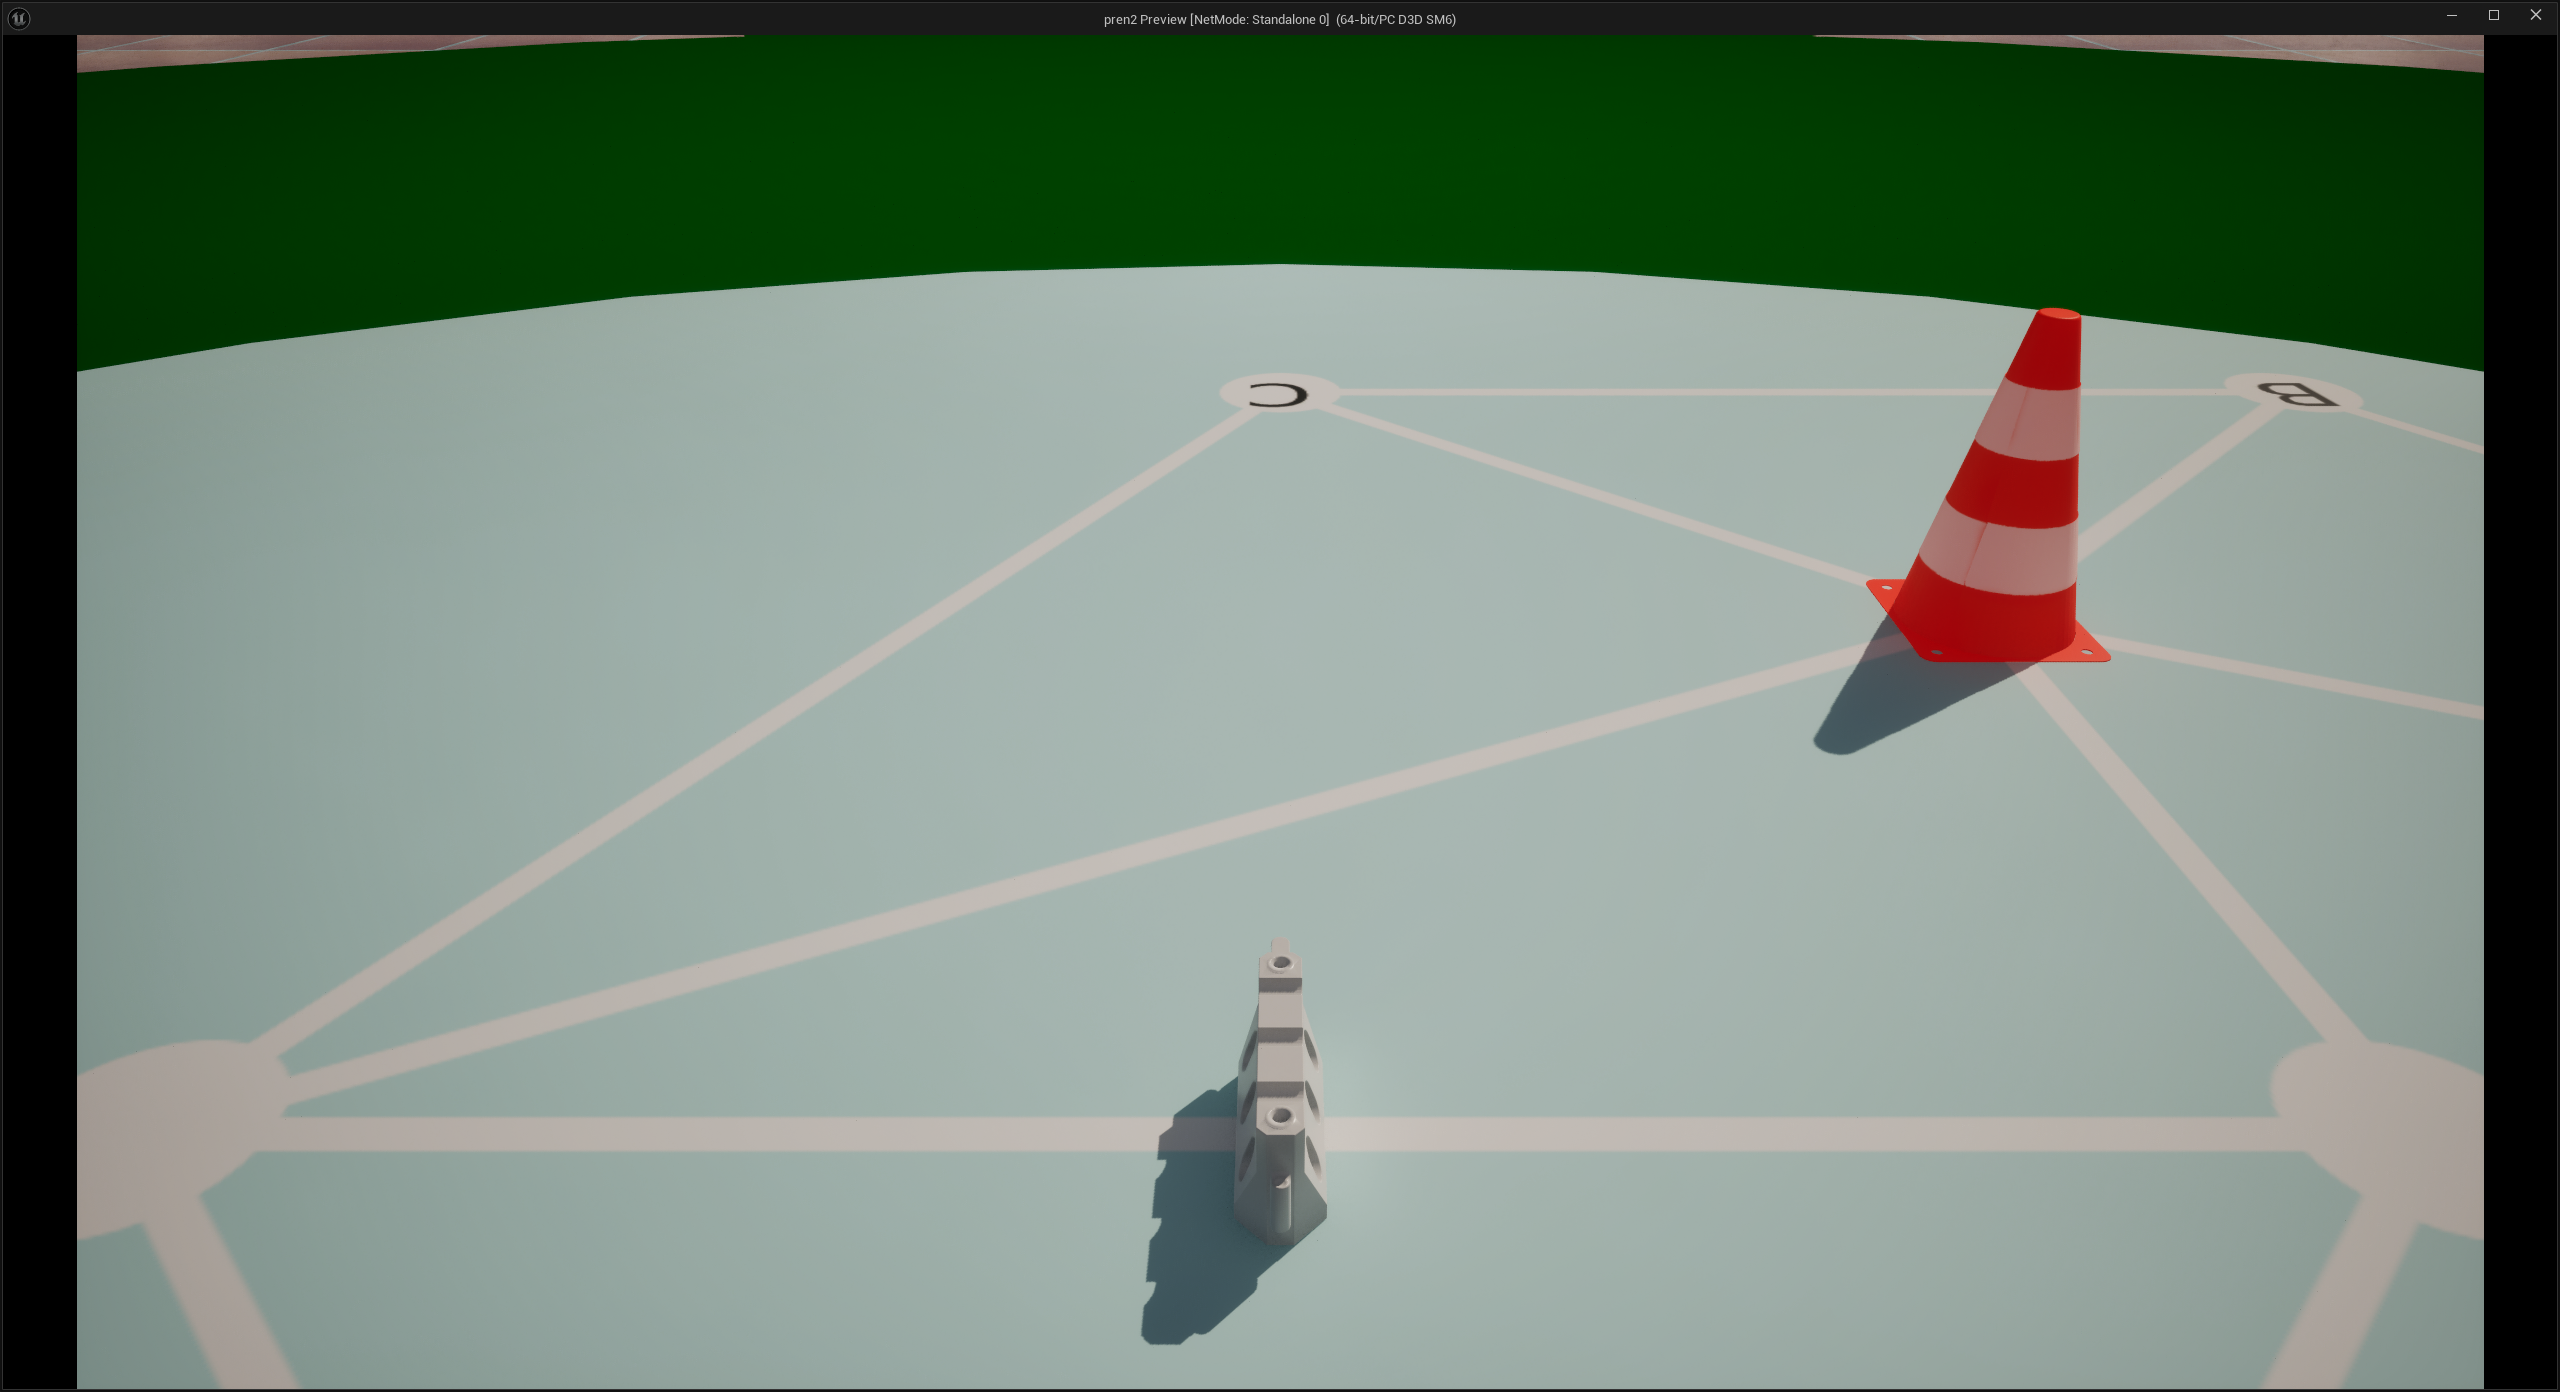
\includegraphics[width=4cm]{img/unrealengine/h50_f75_w30.png} & 
        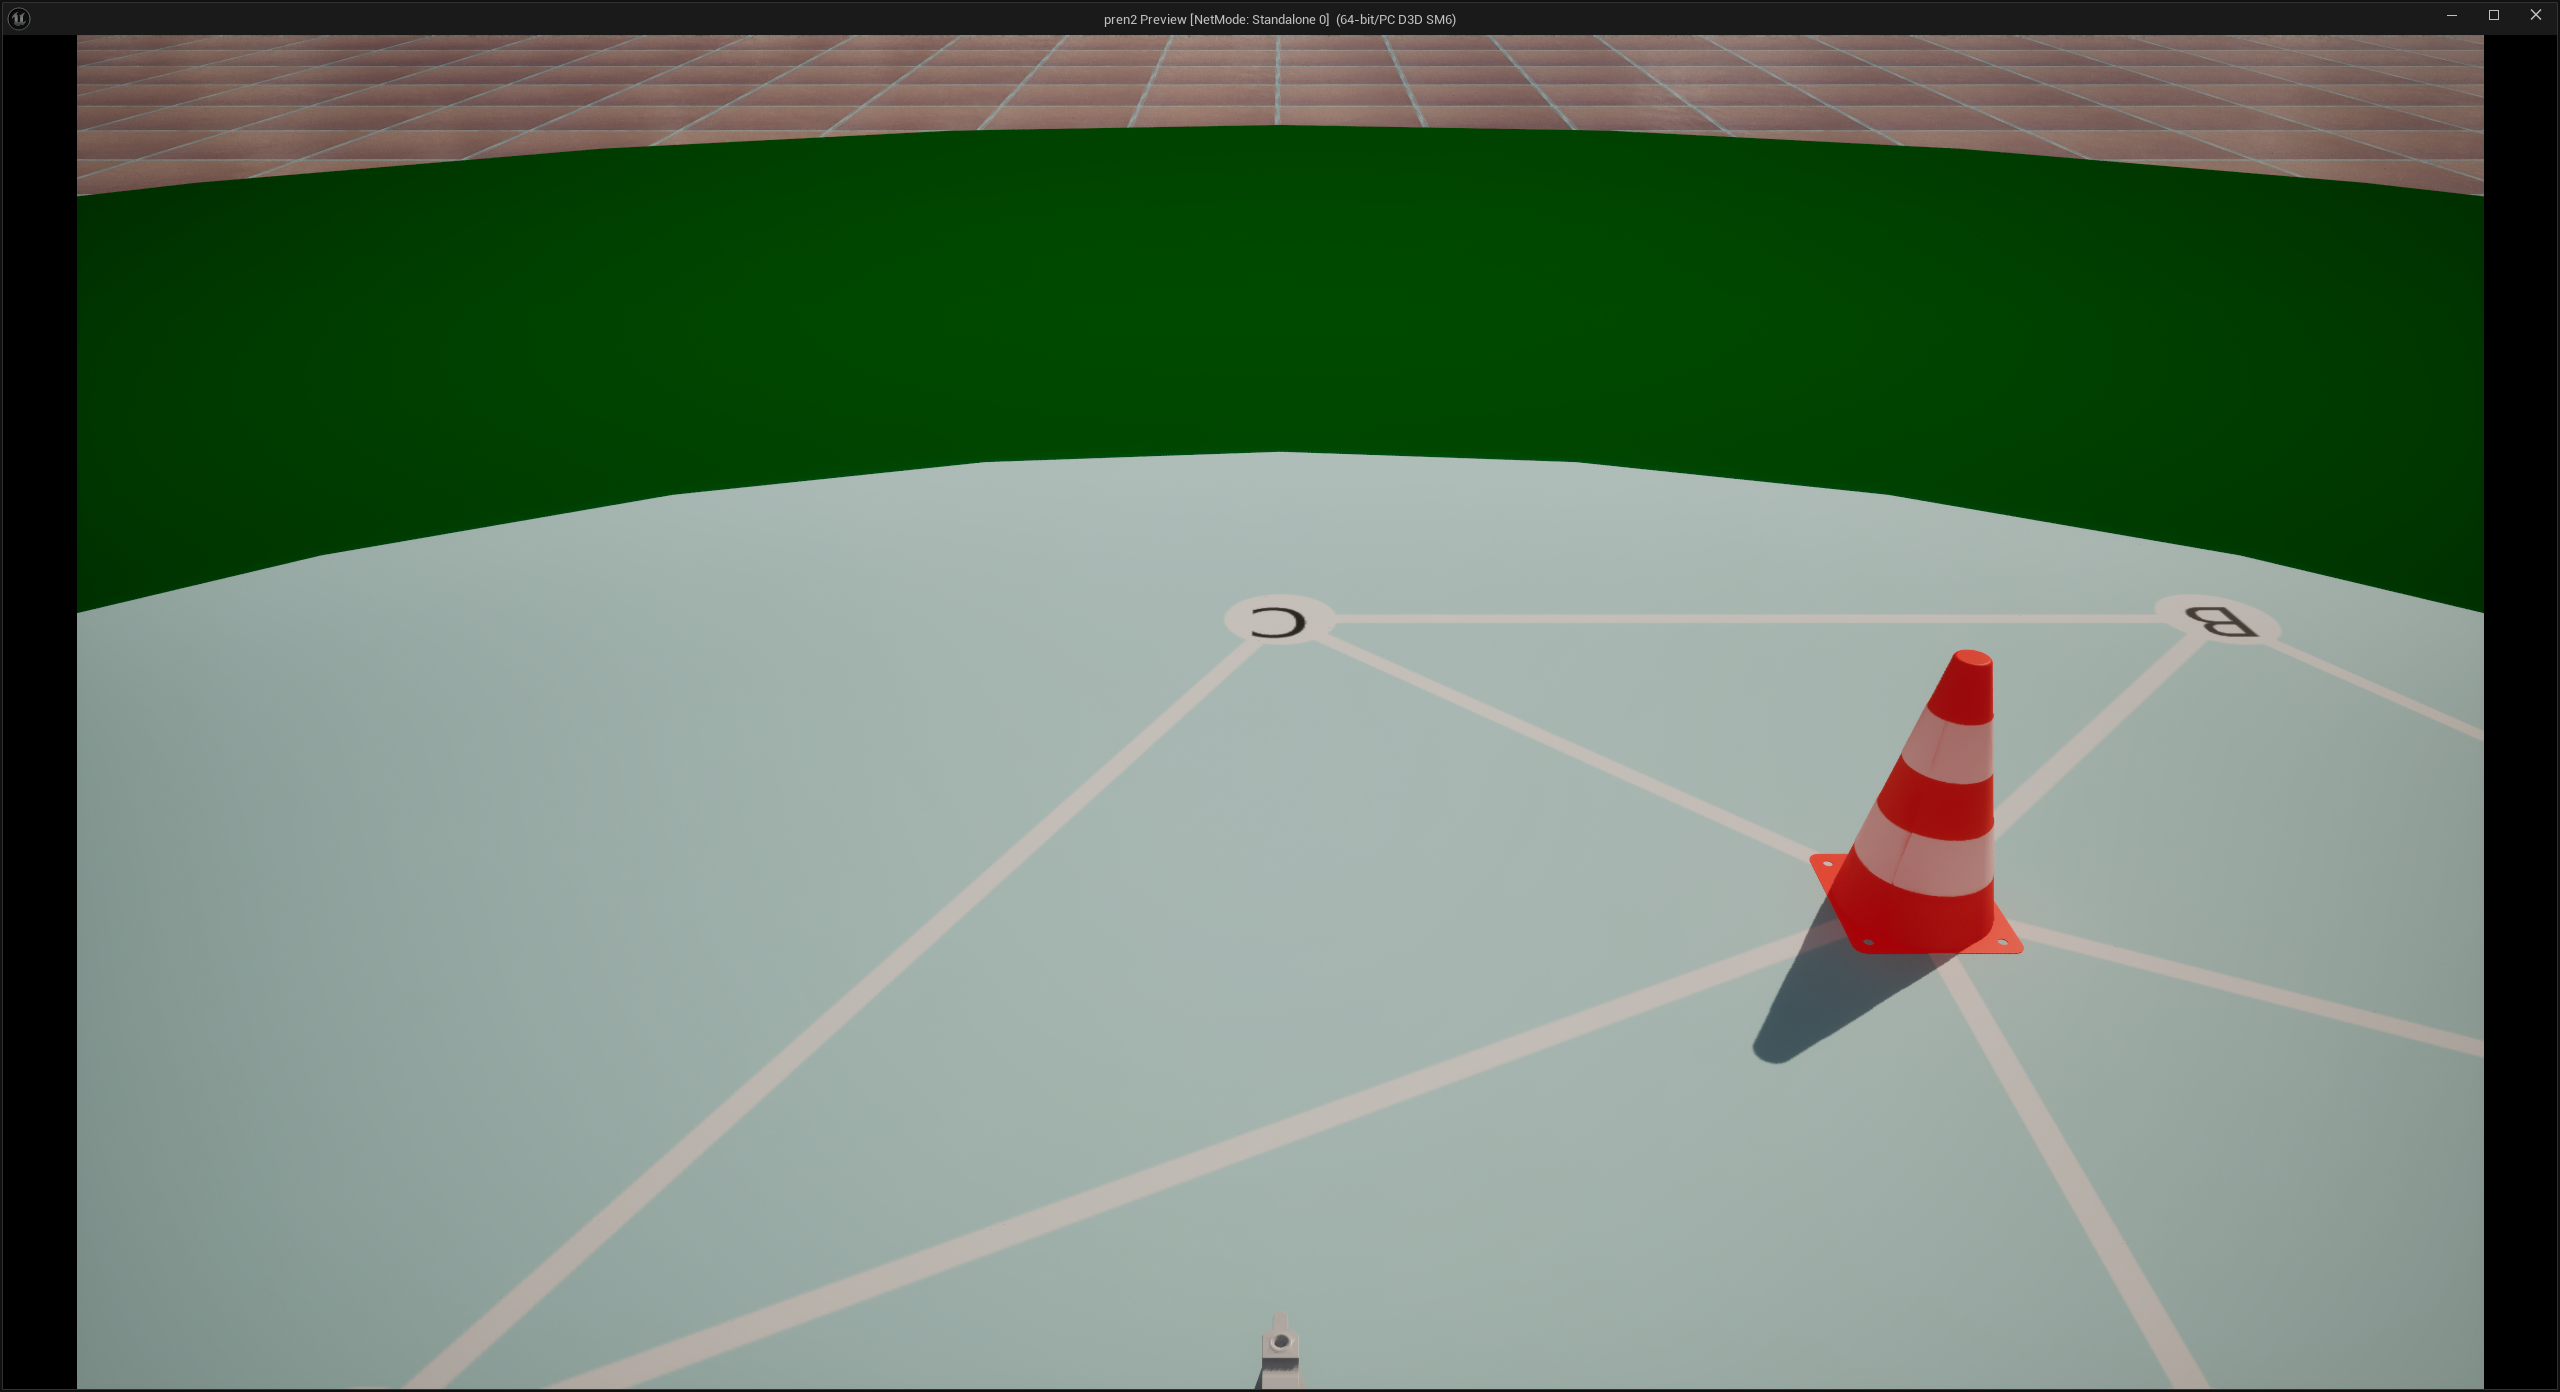
\includegraphics[width=4cm]{img/unrealengine/h75_f75_w30.png} \\
        \hline
        \parbox[c][2cm][c]{4cm}{\centering Kamera FoV 120°, \\ Kameraneigung 45°} & 
        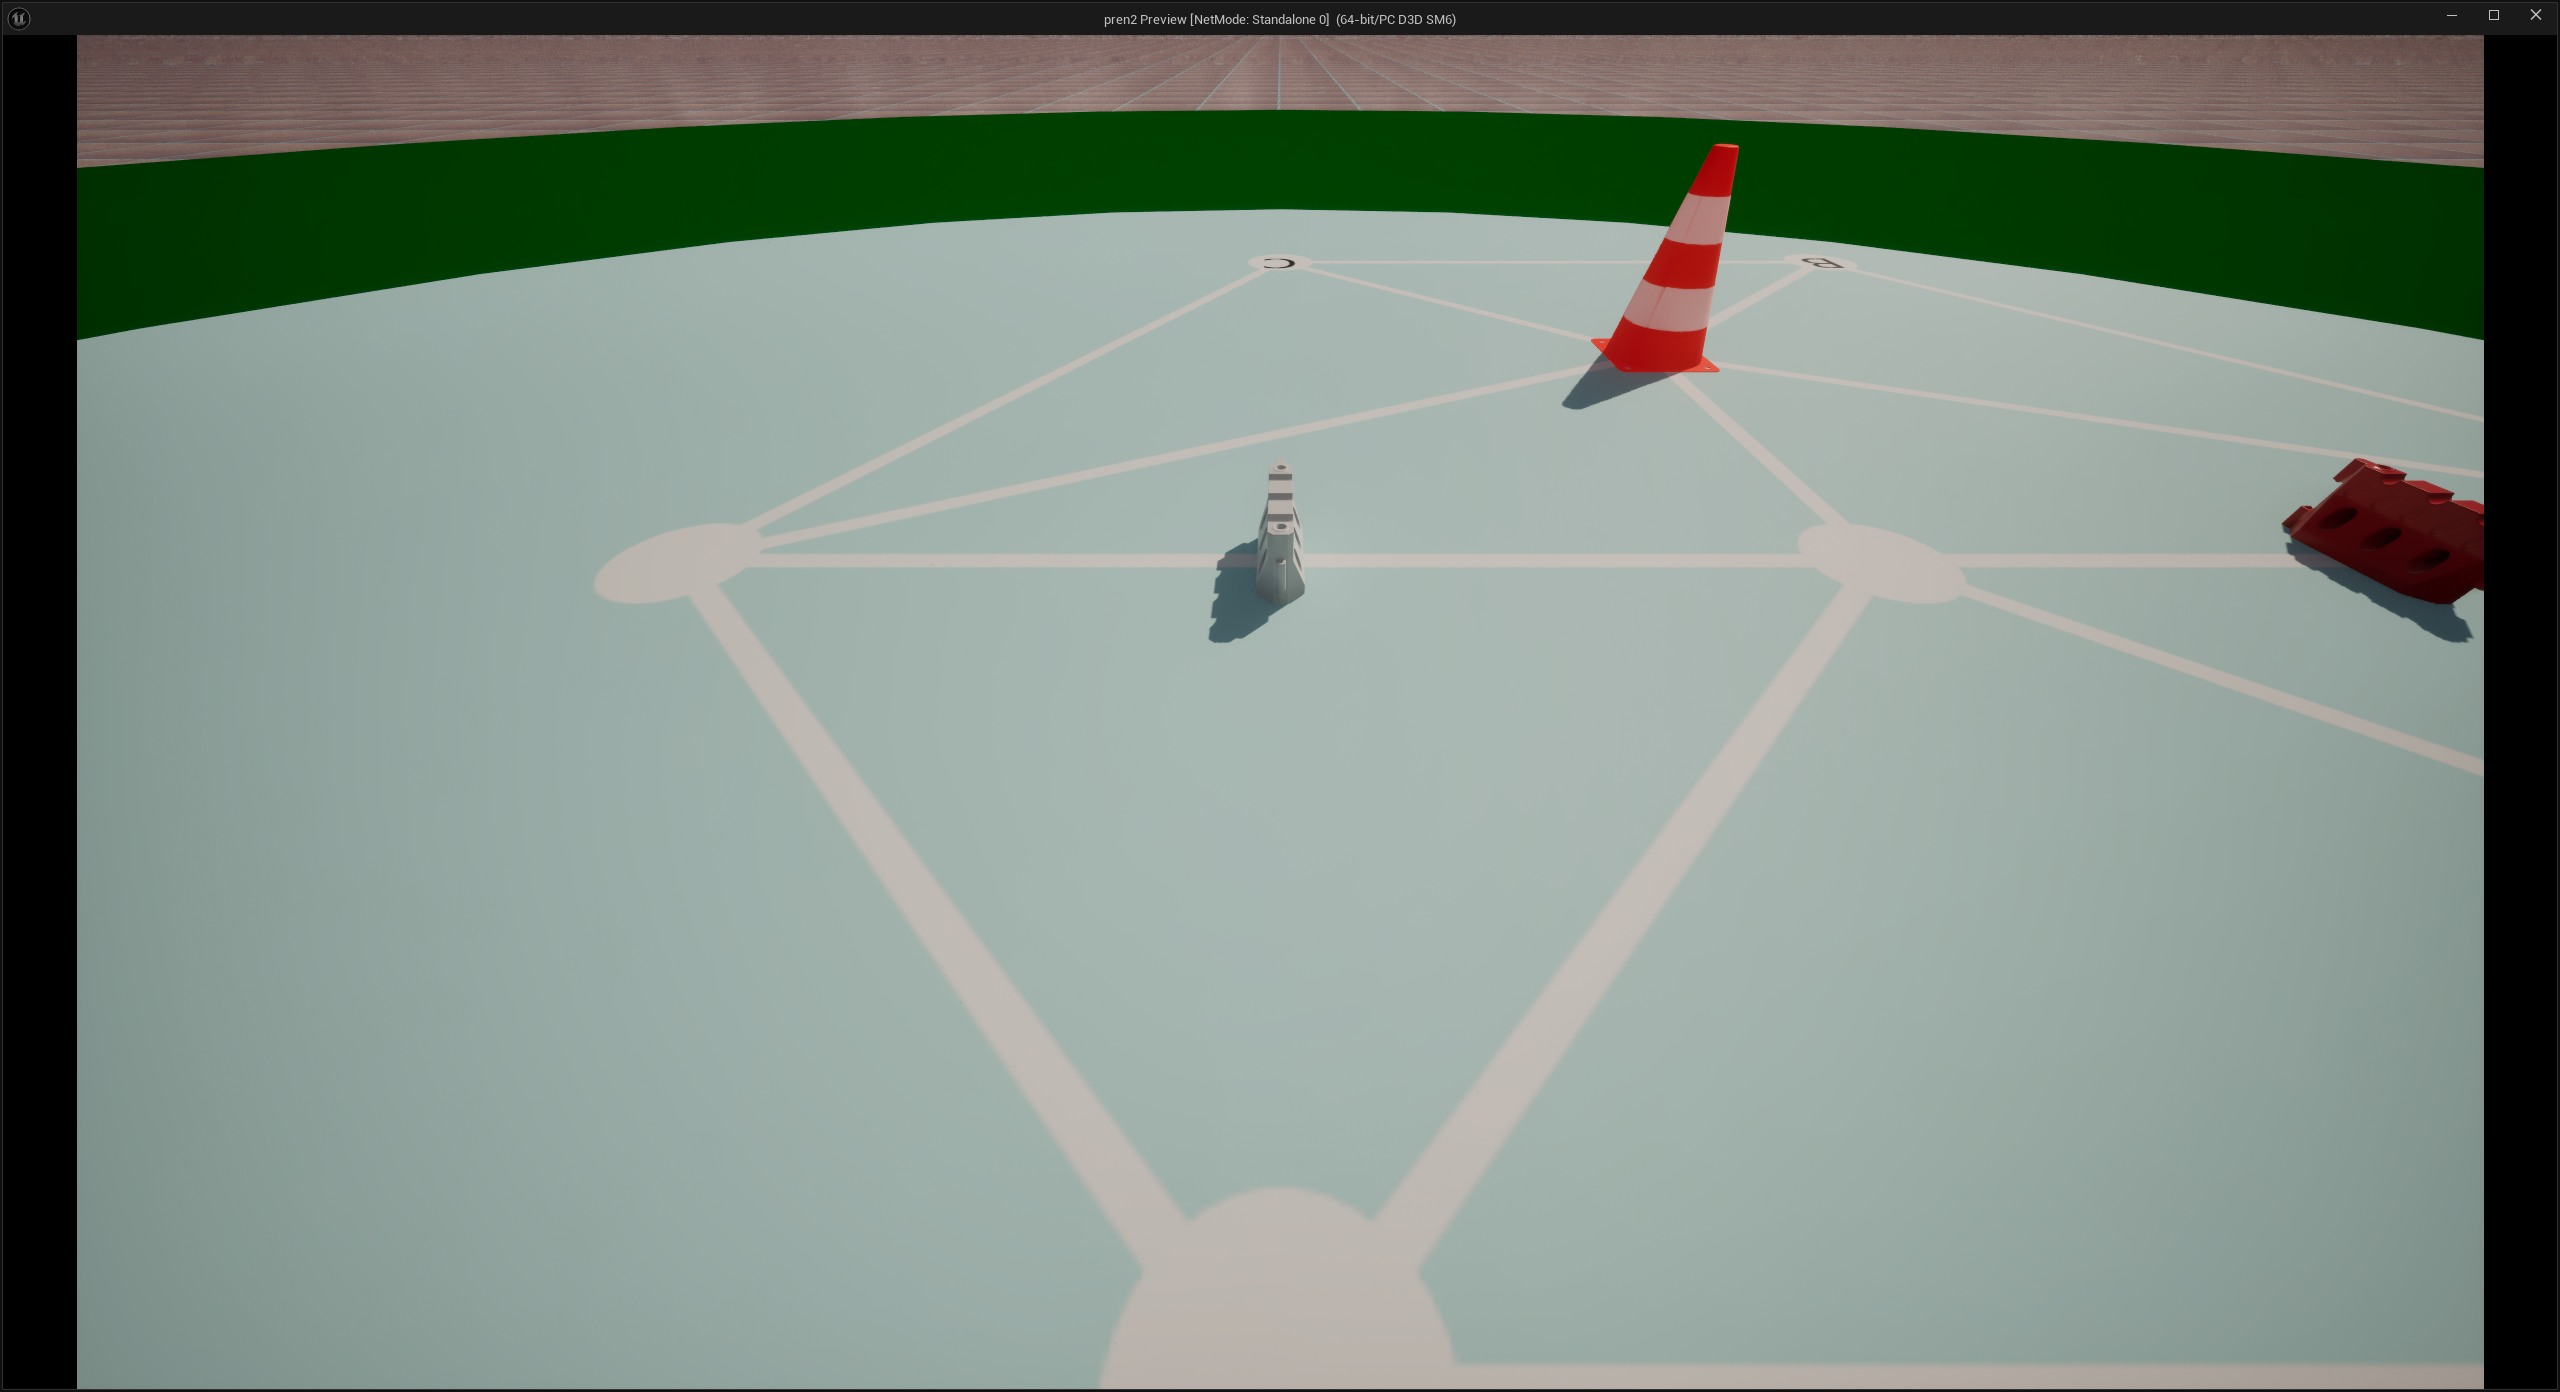
\includegraphics[width=4cm]{img/unrealengine/h30_f120_w45.png} & 
        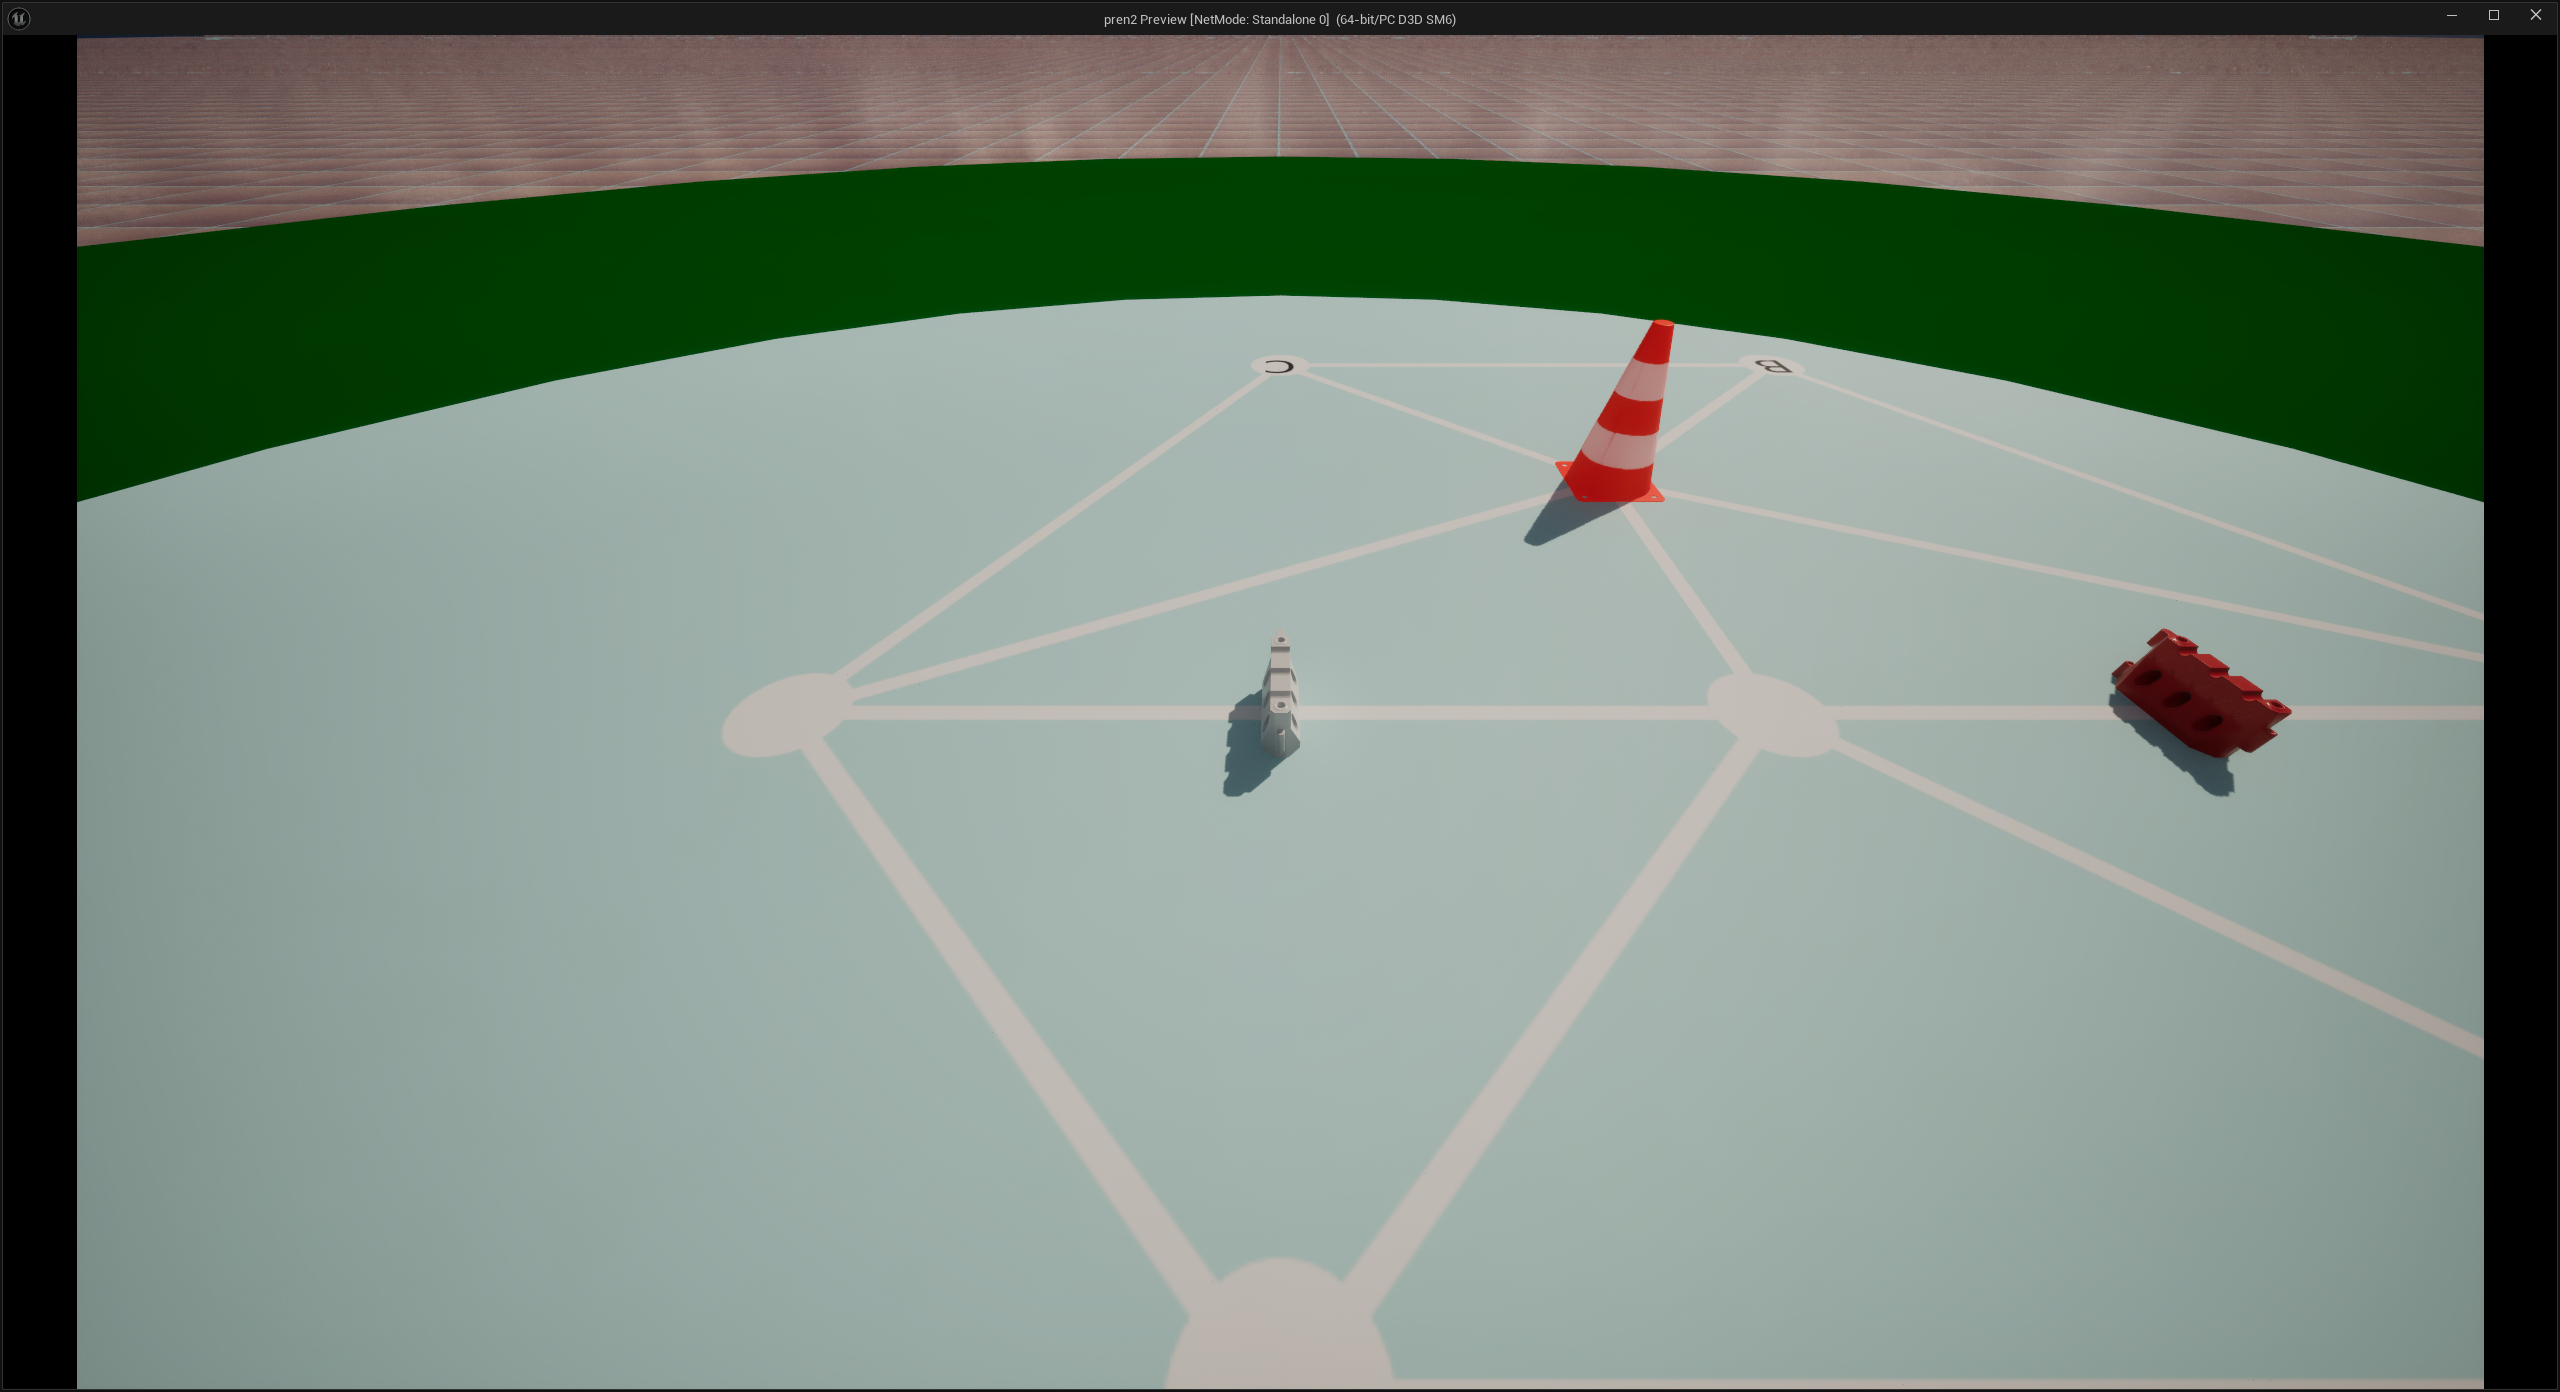
\includegraphics[width=4cm]{img/unrealengine/h50_f120_w45.png} & 
        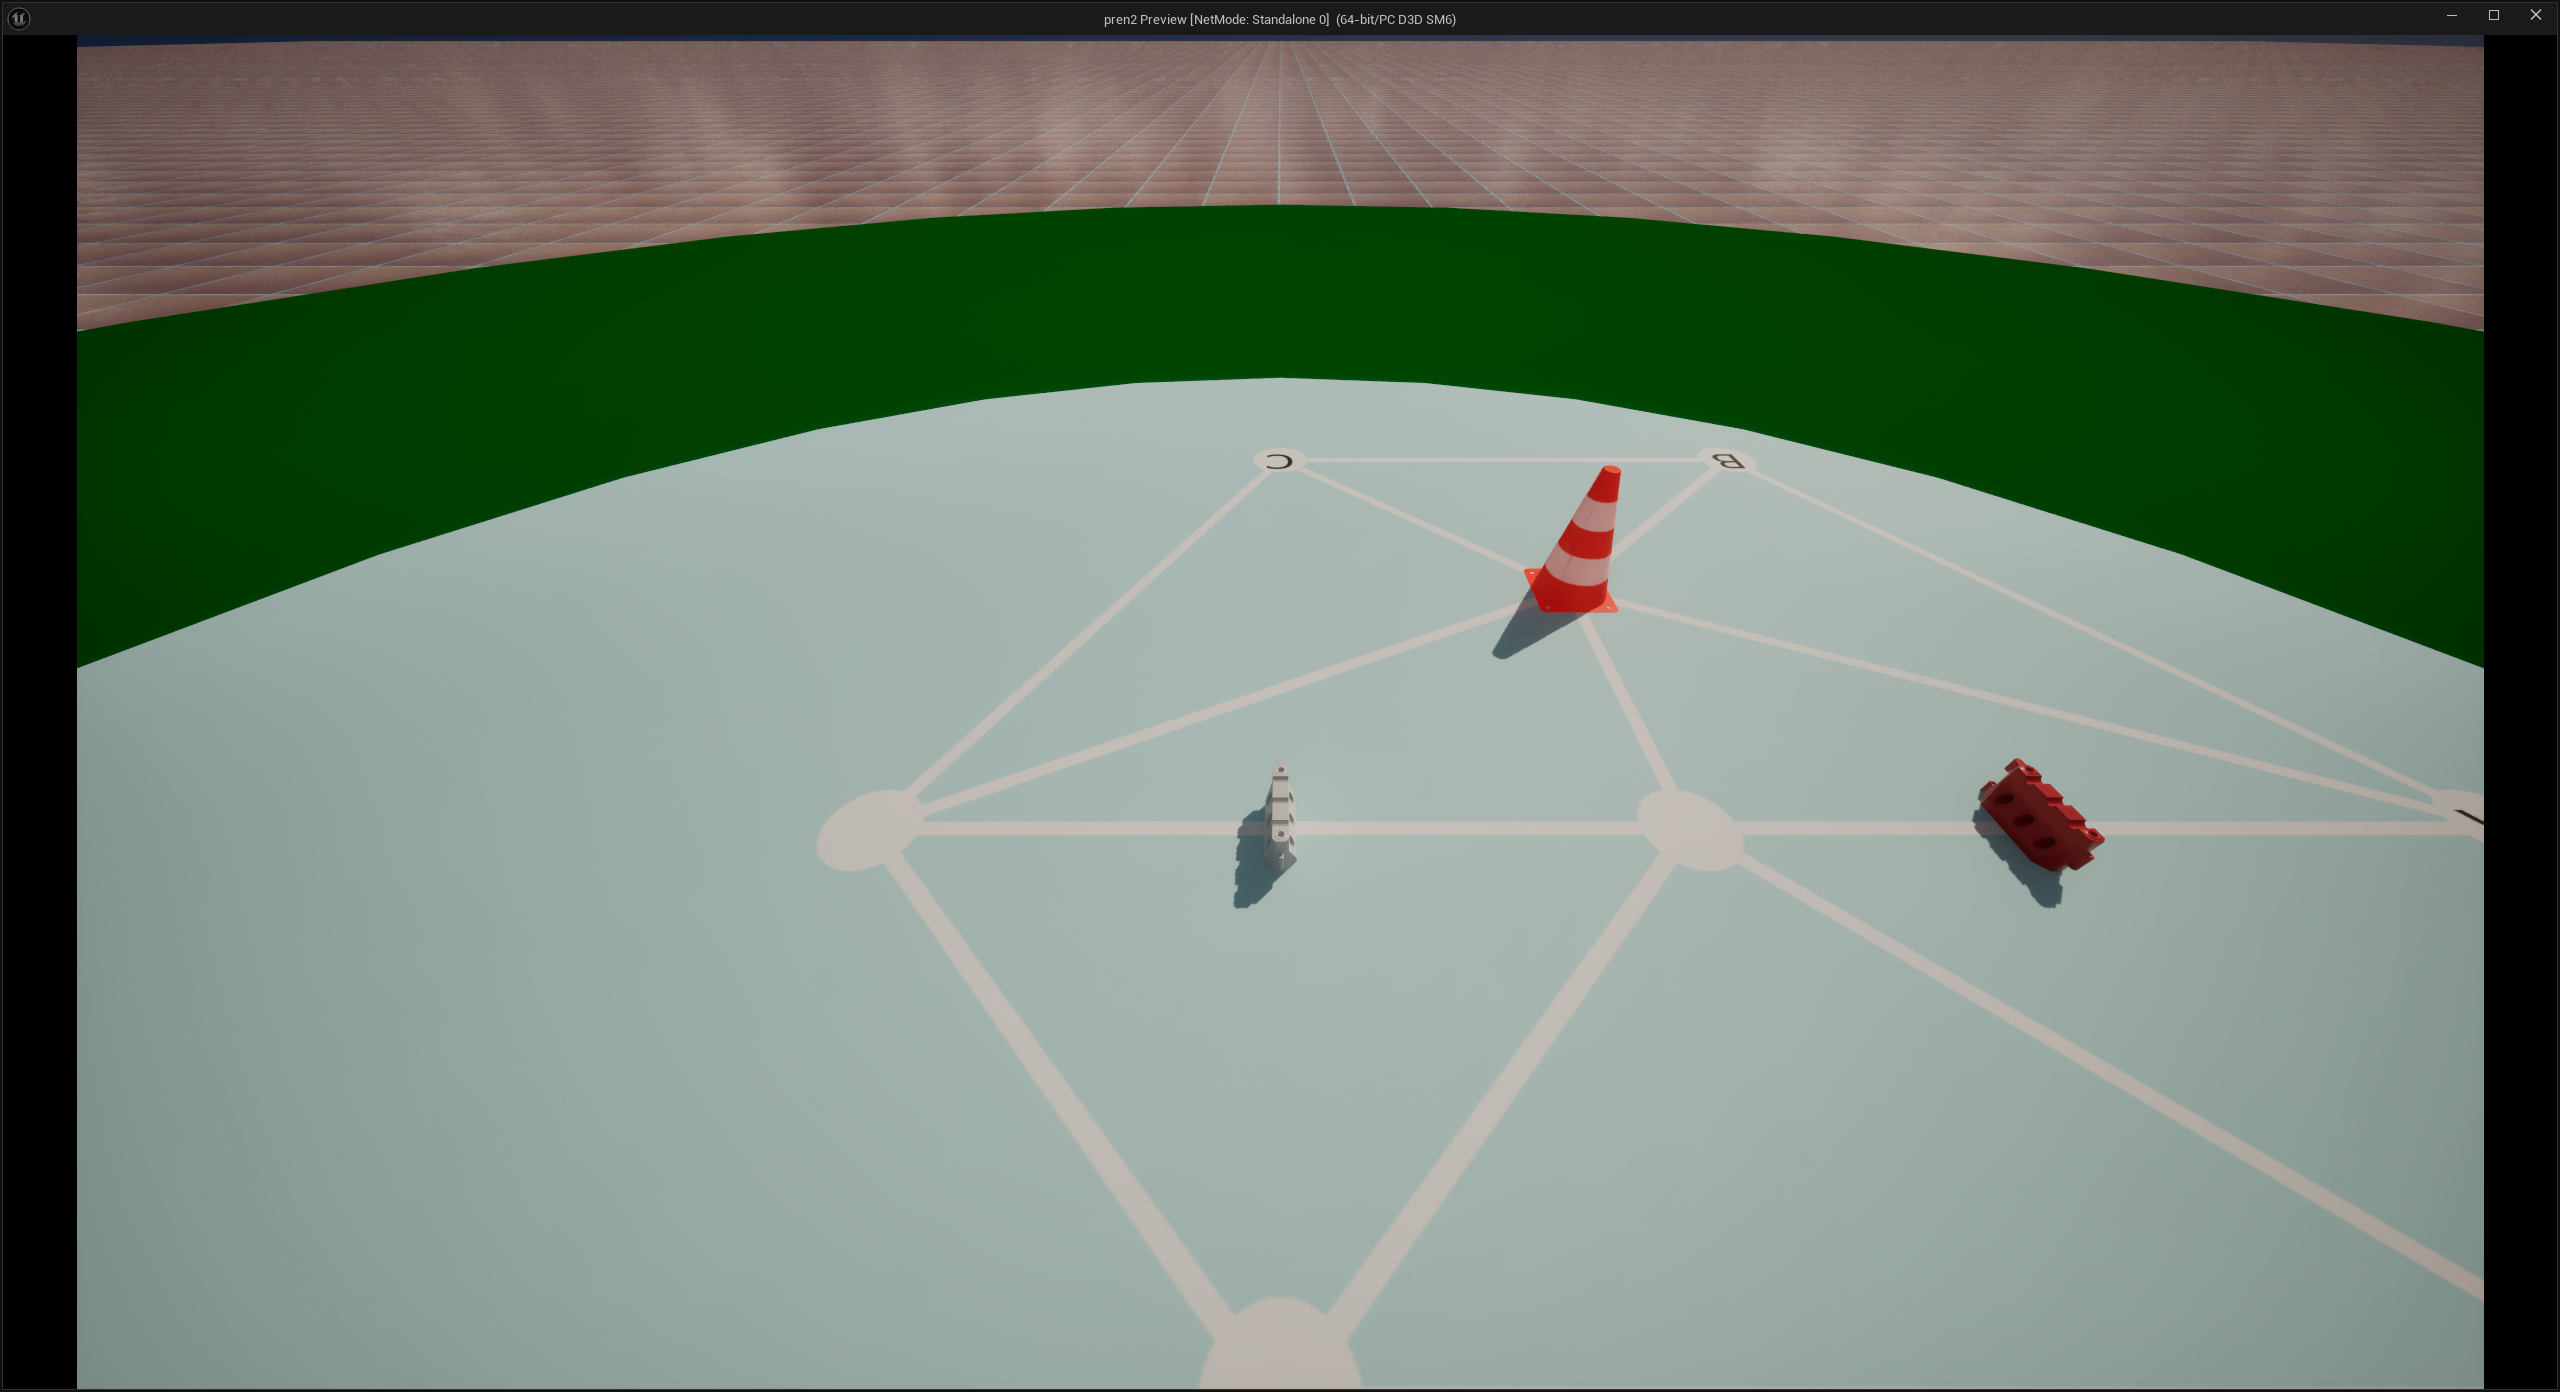
\includegraphics[width=4cm]{img/unrealengine/h75_f120_w45.png} \\
        \hline
    \end{tabular}
    \caption{Vergleich unterschiedlicher Kamera-Einstellungen und Höhen. Der grüne Kreis eine horizontale Distanz von 4.5m von der Kamera entfernt, und der weisse Kreis eine horizontale Distanz von 2m von der Kamera entfernt dar.}
\end{table}


